
%% bare_jrnl.tex
%% V1.4b
%% 2015/08/26
%% by Michael Shell
%% see http://www.michaelshell.org/
%% for current contact information.
%%
%% This is a skeleton file demonstrating the use of IEEEtran.cls
%% (requires IEEEtran.cls version 1.8b or later) with an IEEE
%% journal paper.
%%
%% Support sites:
%% http://www.michaelshell.org/tex/ieeetran/
%% http://www.ctan.org/pkg/ieeetran
%% and
%% http://www.ieee.org/

%%*************************************************************************
%% Legal Notice:
%% This code is offered as-is without any warranty either expressed or
%% implied; without even the implied warranty of MERCHANTABILITY or
%% FITNESS FOR A PARTICULAR PURPOSE!
%% User assumes all risk.
%% In no event shall the IEEE or any contributor to this code be liable for
%% any damages or losses, including, but not limited to, incidental,
%% consequential, or any other damages, resulting from the use or misuse
%% of any information contained here.
%%
%% All comments are the opinions of their respective authors and are not
%% necessarily endorsed by the IEEE.
%%
%% This work is distributed under the LaTeX Project Public License (LPPL)
%% ( http://www.latex-project.org/ ) version 1.3, and may be freely used,
%% distributed and modified. A copy of the LPPL, version 1.3, is included
%% in the base LaTeX documentation of all distributions of LaTeX released
%% 2003/12/01 or later.
%% Retain all contribution notices and credits.
%% ** Modified files should be clearly indicated as such, including  **
%% ** renaming them and changing author support contact information. **
%%*************************************************************************


% *** Authors should verify (and, if needed, correct) their LaTeX system  ***
% *** with the testflow diagnostic prior to trusting their LaTeX platform ***
% *** with production work. The IEEE's font choices and paper sizes can   ***
% *** trigger bugs that do not appear when using other class files.       ***                          ***
% The testflow support page is at:
% http://www.michaelshell.org/tex/testflow/



\documentclass[journal]{IEEEtran}

%\usepackage{algorithm}
%\usepackage{algorithmicx}
%\usepackage{algpseudocode}
%\usepackage{amsmath}

%\renewcommand{\algorithmicrequire}{\textbf{Input:}}  % Use Input in the format of Algorithm
%\renewcommand{\algorithmicensure}{\textbf{Output:}} % Use Output in the format of Algorithm
%
% If IEEEtran.cls has not been installed into the LaTeX system files,
% manually specify the path to it like:
% \documentclass[journal]{../sty/IEEEtran}


\usepackage{latexsym}
\usepackage{amsmath}
\usepackage{amssymb}
\usepackage{graphicx}
\usepackage{subfigure}

\makeatletter
\newif\if@restonecol
\makeatother
\let\algorithm\relax
\let\endalgorithm\relax
\usepackage[linesnumbered,ruled,vlined]{algorithm2e}%[ruled,vlined]{
\usepackage{algpseudocode}
\usepackage{amsmath}
\renewcommand{\algorithmicrequire}{\textbf{Input:}}  % Use Input in the format of Algorithm
\renewcommand{\algorithmicensure}{\textbf{Output:}} % Use Output in the format of Algorithm


% Some very useful LaTeX packages include:
% (uncomment the ones you want to load)


% *** MISC UTILITY PACKAGES ***
%
%\usepackage{ifpdf}
% Heiko Oberdiek's ifpdf.sty is very useful if you need conditional
% compilation based on whether the output is pdf or dvi.
% usage:
% \ifpdf
%   % pdf code
% \else
%   % dvi code
% \fi
% The latest version of ifpdf.sty can be obtained from:
% http://www.ctan.org/pkg/ifpdf
% Also, note that IEEEtran.cls V1.7 and later provides a builtin
% \ifCLASSINFOpdf conditional that works the same way.
% When switching from latex to pdflatex and vice-versa, the compiler may
% have to be run twice to clear warning/error messages.






% *** CITATION PACKAGES ***
%
%\usepackage{cite}
% cite.sty was written by Donald Arseneau
% V1.6 and later of IEEEtran pre-defines the format of the cite.sty package
% \cite{} output to follow that of the IEEE. Loading the cite package will
% result in citation numbers being automatically sorted and properly
% "compressed/ranged". e.g., [1], [9], [2], [7], [5], [6] without using
% cite.sty will become [1], [2], [5]--[7], [9] using cite.sty. cite.sty's
% \cite will automatically add leading space, if needed. Use cite.sty's
% noadjust option (cite.sty V3.8 and later) if you want to turn this off
% such as if a citation ever needs to be enclosed in parenthesis.
% cite.sty is already installed on most LaTeX systems. Be sure and use
% version 5.0 (2009-03-20) and later if using hyperref.sty.
% The latest version can be obtained at:
% http://www.ctan.org/pkg/cite
% The documentation is contained in the cite.sty file itself.






% *** GRAPHICS RELATED PACKAGES ***
%
\ifCLASSINFOpdf
  % \usepackage[pdftex]{graphicx}
  % declare the path(s) where your graphic files are
  % \graphicspath{{../pdf/}{../jpeg/}}
  % and their extensions so you won't have to specify these with
  % every instance of \includegraphics
  % \DeclareGraphicsExtensions{.pdf,.jpeg,.png}
\else
  % or other class option (dvipsone, dvipdf, if not using dvips). graphicx
  % will default to the driver specified in the system graphics.cfg if no
  % driver is specified.
  % \usepackage[dvips]{graphicx}
  % declare the path(s) where your graphic files are
  % \graphicspath{{../eps/}}
  % and their extensions so you won't have to specify these with
  % every instance of \includegraphics
  % \DeclareGraphicsExtensions{.eps}
\fi
% graphicx was written by David Carlisle and Sebastian Rahtz. It is
% required if you want graphics, photos, etc. graphicx.sty is already
% installed on most LaTeX systems. The latest version and documentation
% can be obtained at:
% http://www.ctan.org/pkg/graphicx
% Another good source of documentation is "Using Imported Graphics in
% LaTeX2e" by Keith Reckdahl which can be found at:
% http://www.ctan.org/pkg/epslatex
%
% latex, and pdflatex in dvi mode, support graphics in encapsulated
% postscript (.eps) format. pdflatex in pdf mode supports graphics
% in .pdf, .jpeg, .png and .mps (metapost) formats. Users should ensure
% that all non-photo figures use a vector format (.eps, .pdf, .mps) and
% not a bitmapped formats (.jpeg, .png). The IEEE frowns on bitmapped formats
% which can result in "jaggedy"/blurry rendering of lines and letters as
% well as large increases in file sizes.
%
% You can find documentation about the pdfTeX application at:
% http://www.tug.org/applications/pdftex





% *** MATH PACKAGES ***
%
%\usepackage{amsmath}
% A popular package from the American Mathematical Society that provides
% many useful and powerful commands for dealing with mathematics.
%
% Note that the amsmath package sets \interdisplaylinepenalty to 10000
% thus preventing page breaks from occurring within multiline equations. Use:
%\interdisplaylinepenalty=2500
% after loading amsmath to restore such page breaks as IEEEtran.cls normally
% does. amsmath.sty is already installed on most LaTeX systems. The latest
% version and documentation can be obtained at:
% http://www.ctan.org/pkg/amsmath





% *** SPECIALIZED LIST PACKAGES ***
%
%\usepackage{algorithmic}
% algorithmic.sty was written by Peter Williams and Rogerio Brito.
% This package provides an algorithmic environment fo describing algorithms.
% You can use the algorithmic environment in-text or within a figure
% environment to provide for a floating algorithm. Do NOT use the algorithm
% floating environment provided by algorithm.sty (by the same authors) or
% algorithm2e.sty (by Christophe Fiorio) as the IEEE does not use dedicated
% algorithm float types and packages that provide these will not provide
% correct IEEE style captions. The latest version and documentation of
% algorithmic.sty can be obtained at:
% http://www.ctan.org/pkg/algorithms
% Also of interest may be the (relatively newer and more customizable)
% algorithmicx.sty package by Szasz Janos:
% http://www.ctan.org/pkg/algorithmicx




% *** ALIGNMENT PACKAGES ***
%
%\usepackage{array}
% Frank Mittelbach's and David Carlisle's array.sty patches and improves
% the standard LaTeX2e array and tabular environments to provide better
% appearance and additional user controls. As the default LaTeX2e table
% generation code is lacking to the point of almost being broken with
% respect to the quality of the end results, all users are strongly
% advised to use an enhanced (at the very least that provided by array.sty)
% set of table tools. array.sty is already installed on most systems. The
% latest version and documentation can be obtained at:
% http://www.ctan.org/pkg/array


% IEEEtran contains the IEEEeqnarray family of commands that can be used to
% generate multiline equations as well as matrices, tables, etc., of high
% quality.




% *** SUBFIGURE PACKAGES ***
%\ifCLASSOPTIONcompsoc
%  \usepackage[caption=false,font=normalsize,labelfont=sf,textfont=sf]{subfig}
%\else
%  \usepackage[caption=false,font=footnotesize]{subfig}
%\fi
% subfig.sty, written by Steven Douglas Cochran, is the modern replacement
% for subfigure.sty, the latter of which is no longer maintained and is
% incompatible with some LaTeX packages including fixltx2e. However,
% subfig.sty requires and automatically loads Axel Sommerfeldt's caption.sty
% which will override IEEEtran.cls' handling of captions and this will result
% in non-IEEE style figure/table captions. To prevent this problem, be sure
% and invoke subfig.sty's "caption=false" package option (available since
% subfig.sty version 1.3, 2005/06/28) as this is will preserve IEEEtran.cls
% handling of captions.
% Note that the Computer Society format requires a larger sans serif font
% than the serif footnote size font used in traditional IEEE formatting
% and thus the need to invoke different subfig.sty package options depending
% on whether compsoc mode has been enabled.
%
% The latest version and documentation of subfig.sty can be obtained at:
% http://www.ctan.org/pkg/subfig




% *** FLOAT PACKAGES ***
%
%\usepackage{fixltx2e}
% fixltx2e, the successor to the earlier fix2col.sty, was written by
% Frank Mittelbach and David Carlisle. This package corrects a few problems
% in the LaTeX2e kernel, the most notable of which is that in current
% LaTeX2e releases, the ordering of single and double column floats is not
% guaranteed to be preserved. Thus, an unpatched LaTeX2e can allow a
% single column figure to be placed prior to an earlier double column
% figure.
% Be aware that LaTeX2e kernels dated 2015 and later have fixltx2e.sty's
% corrections already built into the system in which case a warning will
% be issued if an attempt is made to load fixltx2e.sty as it is no longer
% needed.
% The latest version and documentation can be found at:
% http://www.ctan.org/pkg/fixltx2e


%\usepackage{stfloats}
% stfloats.sty was written by Sigitas Tolusis. This package gives LaTeX2e
% the ability to do double column floats at the bottom of the page as well
% as the top. (e.g., "\begin{figure*}[!b]" is not normally possible in
% LaTeX2e). It also provides a command:
%\fnbelowfloat
% to enable the placement of footnotes below bottom floats (the standard
% LaTeX2e kernel puts them above bottom floats). This is an invasive package
% which rewrites many portions of the LaTeX2e float routines. It may not work
% with other packages that modify the LaTeX2e float routines. The latest
% version and documentation can be obtained at:
% http://www.ctan.org/pkg/stfloats
% Do not use the stfloats baselinefloat ability as the IEEE does not allow
% \baselineskip to stretch. Authors submitting work to the IEEE should note
% that the IEEE rarely uses double column equations and that authors should try
% to avoid such use. Do not be tempted to use the cuted.sty or midfloat.sty
% packages (also by Sigitas Tolusis) as the IEEE does not format its papers in
% such ways.
% Do not attempt to use stfloats with fixltx2e as they are incompatible.
% Instead, use Morten Hogholm'a dblfloatfix which combines the features
% of both fixltx2e and stfloats:
%
% \usepackage{dblfloatfix}
% The latest version can be found at:
% http://www.ctan.org/pkg/dblfloatfix




%\ifCLASSOPTIONcaptionsoff
%  \usepackage[nomarkers]{endfloat}
% \let\MYoriglatexcaption\caption
% \renewcommand{\caption}[2][\relax]{\MYoriglatexcaption[#2]{#2}}
%\fi
% endfloat.sty was written by James Darrell McCauley, Jeff Goldberg and
% Axel Sommerfeldt. This package may be useful when used in conjunction with
% IEEEtran.cls'  captionsoff option. Some IEEE journals/societies require that
% submissions have lists of figures/tables at the end of the paper and that
% figures/tables without any captions are placed on a page by themselves at
% the end of the document. If needed, the draftcls IEEEtran class option or
% \CLASSINPUTbaselinestretch interface can be used to increase the line
% spacing as well. Be sure and use the nomarkers option of endfloat to
% prevent endfloat from "marking" where the figures would have been placed
% in the text. The two hack lines of code above are a slight modification of
% that suggested by in the endfloat docs (section 8.4.1) to ensure that
% the full captions always appear in the list of figures/tables - even if
% the user used the short optional argument of \caption[]{}.
% IEEE papers do not typically make use of \caption[]'s optional argument,
% so this should not be an issue. A similar trick can be used to disable
% captions of packages such as subfig.sty that lack options to turn off
% the subcaptions:
% For subfig.sty:
% \let\MYorigsubfloat\subfloat
% \renewcommand{\subfloat}[2][\relax]{\MYorigsubfloat[]{#2}}
% However, the above trick will not work if both optional arguments of
% the \subfloat command are used. Furthermore, there needs to be a
% description of each subfigure *somewhere* and endfloat does not add
% subfigure captions to its list of figures. Thus, the best approach is to
% avoid the use of subfigure captions (many IEEE journals avoid them anyway)
% and instead reference/explain all the subfigures within the main caption.
% The latest version of endfloat.sty and its documentation can obtained at:
% http://www.ctan.org/pkg/endfloat
%
% The IEEEtran \ifCLASSOPTIONcaptionsoff conditional can also be used
% later in the document, say, to conditionally put the References on a
% page by themselves.




% *** PDF, URL AND HYPERLINK PACKAGES ***
%
%\usepackage{url}
% url.sty was written by Donald Arseneau. It provides better support for
% handling and breaking URLs. url.sty is already installed on most LaTeX
% systems. The latest version and documentation can be obtained at:
% http://www.ctan.org/pkg/url
% Basically, \url{my_url_here}.




% *** Do not adjust lengths that control margins, column widths, etc. ***
% *** Do not use packages that alter fonts (such as pslatex).         ***
% There should be no need to do such things with IEEEtran.cls V1.6 and later.
% (Unless specifically asked to do so by the journal or conference you plan
% to submit to, of course. )


% correct bad hyphenation here
\hyphenation{op-tical net-works semi-conduc-tor}


\begin{document}
%
% paper title
% Titles are generally capitalized except for words such as a, an, and, as,
% at, but, by, for, in, nor, of, on, or, the, to and up, which are usually
% not capitalized unless they are the first or last word of the title.
% Linebreaks \\ can be used within to get better formatting as desired.
% Do not put math or special symbols in the title.
\title{Decentralized Task Collaboration for Multiagent System with Compact Coupled Tasks\\ under LTL Specifications}
%
%
% author names and IEEE memberships
% note positions of commas and nonbreaking spaces ( ~ ) LaTeX will not break
% a structure at a ~ so this keeps an author's name from being broken across
% two lines.
% use \thanks{} to gain access to the first footnote area
% a separate \thanks must be used for each paragraph as LaTeX2e's \thanks
% was not built to handle multiple paragraphs
%

\author{Michael~Shell,~\IEEEmembership{Member,~IEEE,}
        John~Doe,~\IEEEmembership{Fellow,~OSA,}
        and~Jane~Doe,~\IEEEmembership{Life~Fellow,~IEEE}% <-this % stops a space
\thanks{M. Shell was with the Department
of Electrical and Computer Engineering, Georgia Institute of Technology, Atlanta,
GA, 30332 USA e-mail: (see http://www.michaelshell.org/contact.html).}% <-this % stops a space
\thanks{J. Doe and J. Doe are with Anonymous University.}% <-this % stops a space
\thanks{Manuscript received April 19, 2005; revised August 26, 2015.}}

% note the % following the last \IEEEmembership and also \thanks -
% these prevent an unwanted space from occurring between the last author name
% and the end of the author line. i.e., if you had this:
%
% \author{....lastname \thanks{...} \thanks{...} }
%                     ^------------^------------^----Do not want these spaces!
%
% a space would be appended to the last name and could cause every name on that
% line to be shifted left slightly. This is one of those "LaTeX things". For
% instance, "\textbf{A} \textbf{B}" will typeset as "A B" not "AB". To get
% "AB" then you have to do: "\textbf{A}\textbf{B}"
% \thanks is no different in this regard, so shield the last } of each \thanks
% that ends a line with a % and do not let a space in before the next \thanks.
% Spaces after \IEEEmembership other than the last one are OK (and needed) as
% you are supposed to have spaces between the names. For what it is worth,
% this is a minor point as most people would not even notice if the said evil
% space somehow managed to creep in.



% The paper headers
\markboth{Journal of \LaTeX\ Class Files,~Vol.~14, No.~8, August~2015}%
{Shell \MakeLowercase{\textit{et al.}}: Bare Demo of IEEEtran.cls for IEEE Journals}
% The only time the second header will appear is for the odd numbered pages
% after the title page when using the twoside option.
%
% *** Note that you probably will NOT want to include the author's ***
% *** name in the headers of peer review papers.                   ***
% You can use \ifCLASSOPTIONpeerreview for conditional compilation here if
% you desire.




% If you want to put a publisher's ID mark on the page you can do it like
% this:
%\IEEEpubid{0000--0000/00\$00.00~\copyright~2015 IEEE}
% Remember, if you use this you must call \IEEEpubidadjcol in the second
% column for its text to clear the IEEEpubid mark.



% use for special paper notices
%\IEEEspecialpapernotice{(Invited Paper)}




% make the title area
\maketitle

% As a general rule, do not put math, special symbols or citations
% in the abstract or keywords.
\begin{abstract}
We consider the collaboration under compact coupled task specifications of a multiagent system that consists of heterogeneous groups of homogeneous agents. To fight the extreme computational complexity of centralized multi-agent planning, we propose a decentralized solution, where couple-edge is proposed to eliminate the coupling among compact task and transform the collaboration issue into a local task planning problem. Meanwhile, we adapt the online coordination scheme based on real-time exchange of request and reply messages to ensure the satisfaction of task specifications without central coordination. This adapted online coordination scheme facilitates not only decreasing the total execution cost but also dispatching agents to strive to complete task when part of agents failure. Proposed approach is demonstrated by a simulated scenario of 14 agents under compact coupled task specifications.
\end{abstract}

% Note that keywords are not normally used for peerreview papers.
\begin{IEEEkeywords}
multiagent system, linear temporal logics (LTLs), decentralized collaboration.
\end{IEEEkeywords}






% For peer review papers, you can put extra information on the cover
% page as needed:
% \ifCLASSOPTIONpeerreview
% \begin{center} \bfseries EDICS Category: 3-BBND \end{center}
% \fi
%
% For peerreview papers, this IEEEtran command inserts a page break and
% creates the second title. It will be ignored for other modes.
\IEEEpeerreviewmaketitle



\section{Introduction}
zhao yu guo meng qu bie, you ming que de xian hou shun xv guan xi?buxv yao ren wei ding yi xie zuo dong zuo

wo men de fang fa neng gou jie jue zhi qian guo meng de song ou he, tong guo huan yi zhong sheng ming fang fa,dan shi guo meng de fang fa jiejue bu le zhe ge wen ti,di yi ,xv yao ding yi xie zuo ren wu,di er qiang ou he xing wu fa sheng cheng chu shi lu jing. di san ,online scheme bu shi yong.
% The very first letter is a 2 line initial drop letter followed
% by the rest of the first word in caps.
%
% form to use if the first word consists of a single letter:
% \IEEEPARstart{A}{demo} file is ....
%
% form to use if you need the single drop letter followed by
% normal text (unknown if ever used by the IEEE):
% \IEEEPARstart{A}{}demo file is ....
%
% Some journals put the first two words in caps:
% \IEEEPARstart{T}{his demo} file is ....
%
% Here we have the typical use of a "T" for an initial drop letter
% and "HIS" in caps to complete the first word.
\IEEEPARstart{T}{his} demo file is intended to serve as a ``starter file''
for IEEE journal papers produced under \LaTeX\ using
IEEEtran.cls version 1.8b and later.
% You must have at least 2 lines in the paragraph with the drop letter
% (should never be an issue)
I wish you the best of success.

\hfill mds

\hfill August 26, 2015

\subsection{Subsection Heading Here}
Subsection text here.

% needed in second column of first page if using \IEEEpubid
%\IEEEpubidadjcol

\subsubsection{Subsubsection Heading Here}
Subsubsection text here.


% An example of a floating figure using the graphicx package.
% Note that \label must occur AFTER (or within) \caption.
% For figures, \caption should occur after the \includegraphics.
% Note that IEEEtran v1.7 and later has special internal code that
% is designed to preserve the operation of \label within \caption
% even when the captionsoff option is in effect. However, because
% of issues like this, it may be the safest practice to put all your
% \label just after \caption rather than within \caption{}.
%
% Reminder: the "draftcls" or "draftclsnofoot", not "draft", class
% option should be used if it is desired that the figures are to be
% displayed while in draft mode.
%
%\begin{figure}[!t]
%\centering
%\includegraphics[width=2.5in]{myfigure}
% where an .eps filename suffix will be assumed under latex,
% and a .pdf suffix will be assumed for pdflatex; or what has been declared
% via \DeclareGraphicsExtensions.
%\caption{Simulation results for the network.}
%\label{fig_sim}
%\end{figure}

% Note that the IEEE typically puts floats only at the top, even when this
% results in a large percentage of a column being occupied by floats.


% An example of a double column floating figure using two subfigures.
% (The subfig.sty package must be loaded for this to work.)
% The subfigure \label commands are set within each subfloat command,
% and the \label for the overall figure must come after \caption.
% \hfil is used as a separator to get equal spacing.
% Watch out that the combined width of all the subfigures on a
% line do not exceed the text width or a line break will occur.
%
%\begin{figure*}[!t]
%\centering
%\subfloat[Case I]{\includegraphics[width=2.5in]{box}%
%\label{fig_first_case}}
%\hfil
%\subfloat[Case II]{\includegraphics[width=2.5in]{box}%
%\label{fig_second_case}}
%\caption{Simulation results for the network.}
%\label{fig_sim}
%\end{figure*}
%
% Note that often IEEE papers with subfigures do not employ subfigure
% captions (using the optional argument to \subfloat[]), but instead will
% reference/describe all of them (a), (b), etc., within the main caption.
% Be aware that for subfig.sty to generate the (a), (b), etc., subfigure
% labels, the optional argument to \subfloat must be present. If a
% subcaption is not desired, just leave its contents blank,
% e.g., \subfloat[].


% An example of a floating table. Note that, for IEEE style tables, the
% \caption command should come BEFORE the table and, given that table
% captions serve much like titles, are usually capitalized except for words
% such as a, an, and, as, at, but, by, for, in, nor, of, on, or, the, to
% and up, which are usually not capitalized unless they are the first or
% last word of the caption. Table text will default to \footnotesize as
% the IEEE normally uses this smaller font for tables.
% The \label must come after \caption as always.
%
%\begin{table}[!t]
%% increase table row spacing, adjust to taste
%\renewcommand{\arraystretch}{1.3}
% if using array.sty, it might be a good idea to tweak the value of
% \extrarowheight as needed to properly center the text within the cells
%\caption{An Example of a Table}
%\label{table_example}
%\centering
%% Some packages, such as MDW tools, offer better commands for making tables
%% than the plain LaTeX2e tabular which is used here.
%\begin{tabular}{|c||c|}
%\hline
%One & Two\\
%\hline
%Three & Four\\
%\hline
%\end{tabular}
%\end{table}


% Note that the IEEE does not put floats in the very first column
% - or typically anywhere on the first page for that matter. Also,
% in-text middle ("here") positioning is typically not used, but it
% is allowed and encouraged for Computer Society conferences (but
% not Computer Society journals). Most IEEE journals/conferences use
% top floats exclusively.
% Note that, LaTeX2e, unlike IEEE journals/conferences, places
% footnotes above bottom floats. This can be corrected via the
% \fnbelowfloat command of the stfloats package.
\section{Preliminaries}

\subsection{Linear Temporal Logic}
Atomic propositions (AP) are boolean variables that can be either true or false and the ingredients of an linear temporal logic are a set of atomic propositions and several boolean and temporal operators, which are specified according to the following syntax[add ref]: $\varphi\ $$:$$:$$=\top|a|\varphi_1\wedge\varphi_2| \neg \varphi|\bigcirc\varphi|\varphi_1\cup\varphi_2|\Box\varphi|\Diamond\varphi|\Longrightarrow\varphi$, where $\top\ (\emph{True})$, $a\ \in AP$, $\bigcirc$ (\emph{Next}), $\cup$ (\emph{Until}), $\Box (\emph{Always})$,  $\Diamond (\emph{Eventually})$ and $\Longrightarrow (\emph{Implicate})$. We refer the readers to [add ref] to grasp the detailed semantics of LTL. We consider $\ \cup\ $, $\Longrightarrow$ and $\wedge$ in this paper which can combine the atomic propositions of different agents, thus generating the compact coupling task.


\subsection{B\"{u}chi Automaton}
Given a LTL formula $\varphi$, we can always translate it to a Nondeterministic B\"{u}chi Automaton (NBA) $\mathcal{A}_\varphi$ that accepts all the languages that satisfy $\varphi$. It is defined as $\mathcal{B}_\varphi=\ (Q,2^{AP},\delta,Q_0,\mathcal{F})$, where $Q$ is a finite set of all the states of B\"{u}chi Automaton, $2^{AP}$ is the set of alphabets, $\delta:\ Q\times 2^{AP}\rightarrow 2^Q$ is the transition relation and $\mathcal{F}\subseteq Q$ is the set of accepting states of B\"{u}chi Automaton. There are fast translation algorithms[add ref] to obtain $\mathcal{B}_\varphi$ from LTL formula $\varphi$.

\section{Problem Formulation}
We consider a multiagent system organized by $N\geq1$ agents. Each agent has the capabilities of navigating within the workspace and performing various motions. The agent index is denoted by $\mathcal{I}=\{p_i,i=1,2,...,N\}$. Then, we divide all the agents into different subsets according to their local LTL task specifications, which implies that only agents with the same local LTL task specifications can be divided into one subset. Assume there are $M$ subsets after dividing, denoted by $\mathcal{G}=\{g_j,j=1,2,...,M\}$. $\mathcal{G}$ satisfies: $g_s\subseteq \mathcal{I},\ \cup_{g_t\subseteq \mathcal{G}}g_t\ =\ \mathcal{I}$ and $g_s\cap g_t\ =\ \emptyset$, $\forall g_t,g_s \subseteq \mathcal{G}$.
\subsection{Motion Abstraction}
Each agent only knows a part of the full workspace which guarantees the completeness of local task and collaboration task. Towards each agent, its workspace consists of $L$ partitions, denoted by $\Pi^{p_i}=\{\pi_1,\pi_2,...,\pi_L\}$, assume all the partitions are known by agents a priori. Besides, there is a set of atomic propositions $\digamma^{p_i}$ describing the properties of the workspace of agent $p_i$. According to [add ref], the motion of $p_i$ is modeled as a finite transition system (FTS) as following[add ref]:
$$\mathcal{F}^{p_i}=(\Pi^{p_i},\rightarrow^{p_i},\Pi^{p_i}_0,L^{p_i},\digamma^{p_i})$$
where $\rightarrow^{p_i} \subseteq \Pi \times \Pi$ is the transition relation, $\Pi^{p_i}_0 \subseteq \Pi^{p_i}$ is the initial region, $L^{p_i}:\Pi^{p_i}\rightarrow 2^{\digamma^{p_i}}$ is the labeling function which indicates the properties held by each region. A path of $\mathcal{F}^{p_i}$ is a sequence of regions $\pi_0 \pi_1 ...\pi_s$ where $(\pi_k,\pi_{k+1})\in \rightarrow^{p_i}$, $\forall k=0,1,...,L-1$.
\subsection{Communication Model}
Similar to the communication model in [add ref], the communication network $\mathcal{V}=(\mathcal{N},\mathcal{E}(t))$ at $t>0$, where $\mathcal{N}$ is the set of nodes and $\mathcal{E}(t)\subseteq \mathcal{N} \times \mathcal{N}$ is the set of edges, which has two layers that $\mathcal{E}(t)=\mathcal{E}_1(t)\cup \mathcal{E}_2(t)$. The first layer $\mathcal{E}_1(t)={(p_i,p_j),\forall i,j\in g_t}$ and $\mathcal{E}_2(t)={(p_i,p_j),\forall i\in g_t,\forall j \in g_s, t\neq s}$. The first layer $\mathcal{E}_1(t)$ is static, which indicates that all the agents belong to the same group $g_t$ can always communicate with each other. The second layer $\mathcal{E}_2(t)$ is dynamic, which indicates that it is enabled when there are decentralized collaboration occurs.
\subsection{Complete Agent Model}
Given the NBA $\mathcal{B}^{p_i}$ associated with $\varphi^{p_i}$ and FTS $\mathcal{F}^{p_i}$, the complete agent model $\mathcal{C}^{p_i}$ of $p_i$ is defined as following:
$$\mathcal{C}^{p_i}=\mathcal{B}^{p_i}\otimes \mathcal{C}^{p_i}=(Q^{p_i,\ast},\delta^{p_i},Q^{p_i,\ast}_0,Q^{p_i,\ast}_{\mathcal{F}},W^{p_i,\ast},\tau^{p_i})$$
where $Q^{p_i,\ast}=\Pi^{p_i}\times Q^{p_i}$, $q^{p_i,\ast}=<\pi^{p_i},q^{p_i}>$, $\forall \pi^{p��_i}\in \Pi^{p_i}$, $\forall q^{p_i}\in Q^{p_i}$; $(<\pi^{p_i}_m,q^{p_i}_s>,<\pi^{p_i}_n,q^{p_i}_t>)\in \delta^{p_i}$ if $\pi^{p_i}_m \rightarrow^{p_i} \pi^{p_i}_n$ and $(q^{p_i}_s,L^{p_i}(\pi^{p_i}_m),q^{p_i}_t)\in \delta^{p_i}$; $Q^{p_i,\ast}_0=\Pi^{p_i}_0\times Q_0^{p_i}$ is the set of initial states; $Q^{p_i,\ast}_{\mathcal{F}}=\Pi^{p_i}\times Q^{p_i}_\mathcal{F}$ is the set of accepting states; $W^{p_i,\ast}:\delta^{p_i}\times Q^{p_i,\ast}\rightarrow \mathbb{R}^{+}$. $W^{p_i,\ast}(<\pi^{p_i}_m,q^{p_i}_s>,<\pi^{p_i}_n,q^{p_i}_t>)=T^{p_i}(\pi^{p_i}_m,\pi^{p_i}_n)$ which is estimated by agent $p_i$, where $<\pi^{p_i}_n,q^{p_i}_t>\in \delta^{p_i}(<\pi^{p_i}_m,q^{p_i}_s>)$. $\tau^{p_i}$ indicates whether $(<\pi^{p_i}_m,q^{p_i}_s>,<\pi^{p_i}_n,q^{p_i}_t>)$ is a couple edge which is going to be introduced next.
\subsection{Compact Coupled Task Specification}
In this paper we consider the compact coupled task specification. Compared to loosely coupled task specifications, compact coupled task specifications relevant to the motions of two or more agents tightly, thus can't be translated to B\"{u}chi Automaton only according to the local agent model and action specification as previous method[add ref]. The compact coupled task specification takes an recursive definition as following.
\par
\emph{Definition 1:} Given a LTL formula $\varphi$ contains temporal operators such as $\cup \ $, $\Longrightarrow$ and  $\wedge$, we denote the terms around each temporal operators by $t^{left}_i$ and $t^{right}_i$, respectively. if $t^{left}_i$ and $t^{right}_i$ belongs to $AP$ of different agents or one of them is a compact coupled task specification, then we say $\varphi$ is a compact coupled task specification.
\par
In other words, a compact coupled task specification should combine the motions of different agents through $\cup \ $, $\Longrightarrow \ $, $\wedge$ so that we can't translate it to B\"{u}chi Automaton and synthesize an initial motion plan for each agent. In summary, we consider following problem.
\par
\emph{Problem 1:}  Given the complete agent model $\mathcal{C}^{p_i}$ and a serious of task specifications $\varphi$ which contain compact coupled task specifications, design a decentralized collaboration scheme such that $\varphi$ is fulfilled for all $p_i \ \subseteq \ \mathcal{I}$.
\section{Decentralized Initial Plan Synthesis}
In this section, we will demonstrate how we decouple the compact coupled task specifications through a set of special edge called couple-edge. Then we use the decoupled B\"{u}chi Automaton to synthesize an initial motion plan for each agent.
\subsection{Decoupling the Compact Coupled Task}
We consider the basic compact coupled task such as $\varphi_1 \cup (\varphi_2 \wedge \varphi_3)$ and $\varphi_1 \Longrightarrow \bigcirc(\varphi_2 \wedge \varphi_3)$, the nested compact coupled task can be transform to basic terms through utilizing auxiliary words. For example, we can transform $\varphi_1 \cup (\varphi_2 \Longrightarrow \bigcirc \varphi_3)$ into $\varphi_1 \cup \kappa$ and $\kappa=\varphi_2 \Longrightarrow \bigcirc \varphi_3$.
\par
Towards basic compact coupled task specification, we notice that compact coupling only exists in the task cooperation process and neither the motions nor states of agent directly participate in the construction of complete models of other agents. For example, consider compact coupled task specification $\neg \varphi_1\cup\varphi_2$, according to definition 1, $\varphi_1$ and $\varphi_2$ belongs to different complete agent models. Consider the local complete agent model $\mathcal{C}^{p_i}$, of which the state set is $Q_c^{p_i}$ that $\varphi_1 \in Q_c^{p_i}|_{\mathcal{M}}$, and $\varphi_2 \notin Q_c^{p_i}|_{\mathcal{M}} $. There exists a subset of $Q_c^{p_i}$ denoted by $\epsilon$ that $\varphi_1 \in \epsilon |_{\mathcal{M}}$ and $\varphi_1 \notin Q_c^{p_i} \setminus \epsilon |_{\mathcal{M}}$. Then there is no edge from $Q_c^{p_i} \setminus \epsilon$ to $\epsilon$ so that we can't synthesize an initial motion plan fulfill $\varphi$.\par
\emph{Definition 2:} Given a complete agent model $\mathcal{C}^{p_i}$, If two nodes $q_i$, $q_j$ satisfy following properties:
\par
(1) $q_i \in \epsilon$, $q_j \in Q_c^{p_i} \setminus \epsilon$ or vice versa.\par
(2) $\delta(q_i,q_j)\subseteq sym(\varphi_c)$ or $\delta(q_j,q_i)\subseteq sym(\varphi_c)$.

where $\varphi_c$ denote the compact coupled part of task specification $\varphi$ and $sym(\varphi)$ denote all the atomic proposition of $\varphi$.
We call each edge which connects $q_i$ and $q_j$ the couple-edge.
At first we can assume that all the collaborative agents have provided assistance and add all the couple-edge to the local complete agent model, then we can synthesize an initial motion plan for each agent.\par
We adapt previous local product algorithm[add ref] which combines the FTS and B\"{u}chi Automaton of single agent for finding out all the couple-edge with respect to the compact coupled task specification $\varphi_c$ and add them into the origin complete agent model. Applying Algorithm 1 we can get a new complete agent model $\mathcal{C}^{p_i}_n$ for each agent, which contains $\mathcal{C}^{p_i}$ and all the couple-edges.\par
\begin{algorithm}
  \caption{Construct New Complete Agent Model $\mathcal{C}^{p_i}_n$}
  \KwIn{the local FTS $\mathcal{F}^{p_i}$, the local B\"{u}chi Automaton $\mathcal{B}^{p_i}$ and the compact coupled task specification $\varphi_c$}
  \KwOut{complete agent model $\mathcal{C}^{p_i}_n$}
  \ForEach{$\pi_i\in \Pi,q_m\in Q$}
  {
    $q'_s=<\pi_i,q_m>\in Q'$

    \If{$\pi_i\in \Pi_0\ and\ q_m\in Q_0$}
    {
        $q'_s\in Q'_0$
    }
    \If{$q_m\in Q_\mathcal{F}$}
    {
        $q'_s\in Q'_\mathcal{F}$
    }
    \ForEach{$\pi_j\in Post(\pi_i),q_n \in Post(q_m)$}
    {
        $q'_g=<\pi_j,q_n>\in Q'$
        $d = CheckTranB(q_m,L_c(\pi_i),q_n,\mathcal{B}^{p_i})$

        \If{$d \geqslant 0$}
        {
            $q'_g\in \delta'(q'_s)$

            $W_p(q'_s,q'_g)=W_c(\pi_i,\pi_j)$

            $\tau(q'_s,q'_g) = None$
        }
        \Else
        {
            \If{$L_c(\pi_i)\in sym(\varphi_c)$}
            {
                $q'_g\in \delta'(q'_s)$

                $W_p(q'_s,q'_g)=W_c(\pi_i,\pi_j)$

                $\tau(q'_s,q'_g)=L_c(\pi_i)$
            }
        }
    }
  }
  \Return $\mathcal{C}^{p_i}_n$
\end{algorithm}

\emph{Lemma 1:} By adding all the couple-edges found out by applying Algorithm 1 to $\mathcal{C}^{p_i}$, we can synthesize an initial accepted motion plan for each agent.\par
\emph{proof:} According to algorithm 1, the nodes in $Q_c^{p_i} \setminus \epsilon$ are connected because these nodes are correspond to independent task specifications. Through adding couple-edges into $\mathcal{C}^{p_i}$, each node in $\epsilon$ becomes reachable and $\mathcal{C}^{p_i}_n$ becomes fully connected. Consequently, there must exist spanning trees for $\mathcal{C}^{p_i}_n$ and there must exist a path from any initial node in $\Phi_0^{p_i}$ to any accepted node in $\Phi_A^{p_i}$. So we can synthesize an initial motion plan fulfilling $\varphi_c$ according to $\mathcal{C}^{p_i}_n$.
\subsection{Plan Synthesis and Reconstitution}
Given $\mathcal{C}^{p_i}_n$ and $\varphi^{p_i}$, there exists a finite path satisfying $\varphi^{p_i}$ if and only if $\mathcal{C}^{p_i}_n$ has a finite path from an initial state to an accepting state. This finite path can be projected back to $\mathcal{F}^{p_i}$ as a finite path. Let $R^{p_i}=q^{p_i}_0 q^{p_i}_1 ... q^{p_i}_s$ be a finite path, where $q^{p_i}_0\in Q_0$, $q^{p_i}_s\in Q_\mathcal{F}$ and $q^{p_i}_z\in Q$ and $(q^{p_i}_z,q^{p_i}_{z+1})\in \delta^{p_i}$. The $cost$ of $R^{p_i}$ is denoted by $cost(R^{p_i},\mathcal{C}^{p_i}_n)=\sum^{s}_{k=0}W^{p_i}(q^{p_i}_k,q^{p_i}_{k+1})$.[add ref] Apply [add ref, Algorithm 1] to find $R^{p_i}$, which utilizes Dijkstra algorithm [add ref] to find the shortest path from any initial state in $Q^{p_i}_0$ to every reachable accepting state in $Q_\mathcal{F}^{p_i}$.

yaobuyao tie ge tu, xing xiang de zhan shi xia suan fa de xiao guo?????????????????????\par
\emph{Lemma 2:} This decentralized initial plan synthesis method has solutions as long as original centralized plan synthesis method has solutions.\par
\emph{Proof:} In algorithm 1 we assume that all the collaborative agents have provided assistance and add all the couple-edges into $\mathcal{C}^{p_i}$. Then towards $\mathcal{C}^{p_i}$, $\varphi_c$ is no longer a constraint. The constraint becomes $\varphi \setminus \varphi_c$. Assume we synthesize an initial motion plan $R$ applying original centralized plan synthesis method, $R$ fulfills $\varphi$ and then $R$ must fulfill $\varphi \setminus \varphi_c$, so all the solutions generated by original centralized method are contained in the solutions generated by decentralized method. Consequently, the proposed decentralized initial plan synthesis method has solutions as long as original centralized plan synthesis method has solutions.\par
$R^{p_i}$ constructed by [zhao na ge suan fa] is composed of prefix $R^{p_i}_p$ and suffix $R^{p_i}_s$. In order to adapt to next algorithms, $R^{p_i}$ is reconstituted as following:\par
(1)Merge $R^{p_i}_p$ and $R^{p_i}_s$ and use $\gamma$ to indicate the separation point.

(2)If two state nodes $q^{p_i}_s$ and $q^{p_i}_t$ satisfy the properties in $\emph{Definition 2}$, add $\delta(q^{p_i}_s,q^{p_i}_t)$ to the attribute $req^{p_i}$ of $q^{p_i}_s$.

\section{Decentralized Task Collaboration}
In previous section, we assume that all the collaborative agents have provided assistance and add all the couple-edges into $\mathcal{C}^{p_i}$, which permits us to synthesize an initial motion plan for each agent. If each agent runs on its own local path independently without any communication with other agents, there may be no guarantee that the collaborative task will be completed, which may result in a violation of the task specification $\varphi$. In response to this issue, we adapt the online coordination scheme to ensure the completion of the collaborative task.
\subsection{Planning In Speed Matching Horizon}
In order to reduce the complexity of task collaboration, we apply a receding horizon method for each agent. Consider the initial reconstituted motion plan $\varrho^{p_i}$ previous, assume the current position of agent $p_i$ is $\pi^{p_i}$ which is the $l$th element of $\varrho^{p_i}$ namely $\varrho^{p_i}[l]$. Assign a receding time $T_H$ for each agent, note that different agents have different velocity so each agent will adjust its velocity according to its speed. Assume that each agent could estimate the approximate time according its current velocity, departure position and target position, then the segment the agent expected to execute in $T_H$ is denoted by $\tau^{p_i}_H$, $\tau^{p_i}_H = \varrho^{p_i}[l:t]$, where the index $t$ is the solution of the following optimization problem: min $t$, subject to $\sum_{k=l}^{t}T^{p_i}(\varrho^{p_i}[k],\varrho^{p_i}[k+1])\geq T_H$, this issue can be solved by iterating through the $\varrho^{p_i}$ and computing the accumulated time which is compared to $T_H$. If previous optimization problem doesn't have a solution, it means that in $T_H$ the agent can execute the rest of the suffix of $\varrho^{p_i}$, namely $\varrho^{p_i}[l:]$. Since the split point of $\varrho^{p_i}$ has been indicated previously, original optimization problem can be transformed into a new optimization problem: min $t$, subject to $\sum_{k=\gamma}^{t}T^{p_i}(\varrho^{p_i}[k],\varrho^{p_i}[k+1])\geq T_H - \sum_{k=l}^{|\varrho^{p_i}|}T^{p_i}(\varrho^{p_i}[k],\varrho^{p_i}[k+1])$, where $|\varrho^{p_i}|$ denote the length of $\varrho^{p_i}$ and $\gamma$ denote the split point index. We can always find a solution to above problem iteratively.

\subsection{Online Coordination Scheme}
Through speed matching receding horizon planning, the truncation index is founded and the receding horizon motion plan $\varrho^{p_i}_H$ is synthesized. To ensure the fulfill of task specification $\varphi$, each agent needs to check whether it needs others' collaboration within $\varrho^{p_i}_H$. Since we have reconstituted the motion plan of each agent, we can just find the first item in $\varrho^{p_i}_H$ which has $req^{p_i}$ attribute.  After one agent confirms that it needs others' collaboration, a $\textbf{Request}^{p_i}$ is sent to others. More specifically, for the first item $<\pi_c^{p_i},req^{p_i}>\ \in \varrho^{p_i}_H$ satisfying $req \neq \emptyset$, where $c$ denote the index of $<\pi_c^{p_i},req^{p_i}>$ in $\varrho^{p_i}_H$. Agent $p_i$ needs to broadcast the request message to $\mathcal{N}^{p_i}$ through its communicate network. $\textbf{Request}^{p_i}$ has the following format:
$$\textbf{Request}^{p_i} = (\chi^{p_i},\pi_c^{p_i},T^{p_i}_e)$$
where $\chi^{p_i}$ denotes all the items in $req^{p_i}$, which indicates the collaborative motion agent $p_i$ needs in $\pi_c^{p_i}$, and $T^{p_i}_e$ denotes the estimated time spent from $\varrho^{p_i}[l]$ to $\varrho^{p_i}[c]$, namely $T^{p_i}_e=\sum_{k=l}^{c}T^{p_i}(\varrho^{p_i}_H[k],\varrho^{p_i}_H[k+1])$. Since $\varrho^{p_i}_H[c]$ is the predecessor of the first request state in $\varrho^{p_i}_H$, $\varrho^{p_i}_H[c]$ can be always reached within finite time, so $T^{p_i}_e$ is a finite positive number.\par
If agent $p_i$ proposes a request message and there is no reply message transitorily, all the collaborations $p_i$ requests are stored in $\mathcal{R}^{p_i}_c$, the current state $\varrho^{p_i}_r$ is stored.\par
The algorithm finding out the first request in receding horizon motion plan $\varrho^{p_i}_H$ is as Algorithm 2.\par
\begin{algorithm}
  \caption{Plan in Horizon and Request}
  \KwIn{$\varrho^{p_i},\pi^{p_i},T_H,\gamma$}
  \KwOut{$\varrho^{p_i}_H,\textbf{Request}^{p_i}$}
  $\varrho^{p_i}[l]=\pi^{p_i},m=0,T_m=0,\textbf{Request}^{p_i}=\emptyset$

  \While{$T_m<T_H$}
  {
    $m=m+1$

    $n=m$

    \If{$m>|\varrho^{p_i}|$}
    {
        $m=\gamma-l$
    }

    $T_m=T_m+T^{p_i}(\varrho^{p_i}[l+n-1],\varrho^{p_i}[l+m])$

    $<\pi^{p_i}_c,req^{p_i}>=\varrho^{p_i}[l+m]$

    \If{$req^{p_i}\neq \emptyset$ and $\textbf{Request}^{p_i}=\emptyset$}
    {
        \ForAll{$\chi^{p_i}\in req^{p_i}$}
        {
            add $(\chi^{p_i},\pi^{p_i}_c,T_m)$ to $\textbf{Request}^{p_i}$
        }
    }
  }
  \If{$m>n$}
  {
    $\varrho^{p_i}_H=\varrho^{p_i}[l:l+m]$
  }
  \Else
  {
    $\varrho^{p_i}_H=\varrho^{p_i}[l:]\oplus \varrho^{p_i}[\gamma:m]$
  }
  \Return $\varrho^{p_i}_H,\textbf{Request}^{p_i}$;
\end{algorithm}
Once there are request messages transmitted among agents, some agents should revise their motion plan to provide assistance. The procedure of determining which agent to respond to the request is quite similar with the algorithm proposed in [add ref], we only present a brief overview here and we refer the readers to [add ref] to grasp more detail. In order to provide collaboration, the collaborative agent needs to revise its motion plan temporarily. Assume current state of agent $p_j$ is $\varrho^{p_j}[l]$ and next accepting state is $\varrho^{p_j}[f]$, original motion plan from $\varrho^{p_j}[l]$ to $\varrho^{p_j}[f]$ is $R^{p_j}_-=\varrho^{p_j}[l:f]$ and the motion plan after revision is denoted by $R^{p_j}_+$, the index of the position in where agent $p_j$ provides collaboration is $m$. We require each agent to calculate the cost of providing assistance in order to decide which agent to collaborate. The $balanced$ cost is defined as following:
\[ \begin{split}
BalCost(R^{p_j}_+,&T^{p_i}_e,\mathcal{C}^{p_j})=\\
&|(\sum_{k=l}^{m}T^{p_j}(\varrho^{p_j}[k],\varrho^{p_j}[k+1])-T^{p_i}_e)|\\
&+\beta_{p_j} \times (Cost(R^{p_j}_+,\mathcal{C}^{p_j})-Cost(R^{p_j}_-,\mathcal{C}^{p_j}))
\end{split} \]
where the first part denotes the time gap between the agent which sends a request message arriving the position where needs collaboration and corresponding agent arrive the position where assistance is provided. Simply, the first part denotes the waiting time of multiagent system, which contains both the waiting time of request agent and reply agent. The second part denotes the additional cost of $R^{p_i}_+$ compared with $R^{p_i}_-$, and $\beta_{p_j}$ is a designed parameter as relative weighting. Instead of formulating the agent choice issue as an integer programming problem,[add ref], we transmit the balanced cost of each agent among the group $\mathcal{N}^{G}$, since each agent calculates its balanced cost in the same way, there must exist a consensus agent $p_{min}$ whose balanced cost is minimal and $p_{min}$ will be elected to reply to corresponding $\textbf{Request}^{p_i}$.\par
After $p_{min}$ is elected, we design an attribute of agent named $state^{p_i}$ which turns into $locked$ when agent $p_i$ is providing collaboration, otherwise $state^{p_i}$ is $normal$. Meanwhile, due to the property of compact coupled task, all the request messages that have time overlapping can be replied by a group of heterogeneous agents. So towards each request message $Request^{p_i}$, if there is already a group of agents ${p_i}$ whose $state^{p_i}$ are $locked$, ${p_i}$ automatically become the collaborative agents and the corresponding request message becomes invisible to other agents.\par
Towards some compact coupled task, such as agents can't across region $r_i$ until some agents reach region $r_j$, only a group of agents is needed to reply request messages from different agents. Hence if two request messages $\textbf{Request}^{p_i}$ and $\textbf{Request}^{p_j}$ have time overlapping and there is a group of agents $\partial$ replying one request messages, then $\partial$ is selected as the reply agents for the other request message $\textbf{Request}'$ and $\textbf{Request}'$ becomes invisible to other agents.\par
$R^{p_i}_+$ can be constructed by the $bidirectional Dijkstra$ algorithm which utilizes the function $bidirectional\_dijkstra()$ in $Networkx$, we refer the readers to [add ref] for more details. After the reply agent $p_r$ is elected, when $p_i$ reaches the requested replying position and provides collaboration, there is a reply message sent from the reply agent to request agent, whose format is as following:
$$\textbf{Reply}^{p_r}=(p_r,p_i,\xi)$$
where $p_r$ denotes the grade of replying agent and $\xi$ denotes the collaboration provided.\par
Finally, we adapt the purpose and structure of $\textbf{Confirm}^{p_i}$ to suit the compact coupled task specification. The format of confirm message is as following:
$$\textbf{Confirm}^{p_i}=(p_i,p_r,\hat{\xi})$$
where $p_r$ denotes the grades of all replying agents and $\hat{\xi}$ denotes that $p_i$ has relieved collaboration requirements for action $\hat{\xi}$. It is sent when the agents which send the request message separate themselves from the area where the collaboration is required and enter next state and the confirm messages informs the replying agents to recovery their $state^{p_r}$ from $locked$ to $normal$. Denote all the request, reply and confirm messages which agent $p_i$ received by $\textbf{Request}_{p_i}^{\ast}$, $\textbf{Reply}_{p_i}^{\ast}$, $\textbf{Confirm}_{p_i}^{\ast}$, respectively. The entire algorithm to handle request, reply and confirm messages is as Algorithm 3.

\begin{algorithm}
  \caption{Handle Reply and Confirm messages}
  \KwIn{$\textbf{Request}_{p_i}^{\ast}$, $\textbf{Reply}_{p_i}^{\ast}$, $\textbf{Confirm}_{p_i}^{\ast}$, $\partial$, $\mathcal{R}^{p_i}_c$, $\mathcal{C}^{p_i}$, assist collaboration $\mathcal{A}^{p_i}_s$ }
  \KwOut{$R^{p_j}_+$}
  $\mathcal{A}^{p_i}_s=\emptyset$

  \If{$\textbf{Request}_{p_i}^{\ast} \neq \emptyset$}
  {
    \ForEach{$\textbf{Request}^{r} = (\chi^{r},\pi_c^{r},T^{r}_e) \in \textbf{Request}_{p_i}^{\ast}$}
    {
        \If{$\partial \neq \emptyset\ and\ p_i \notin \partial$ }
        {
            continue
        }
        \ElseIf{$(\partial \neq \emptyset\ and\ p_i \in \partial)$ or $(\partial = \emptyset\ and\ min_{\mathcal{N}^G}BalCost = p_i)$}
        {
            $(R^{p_i}_+,b^{p_i}_d,t^{p_i}_d)=EvalReq(R^{p_i}_-,(\chi^{p_i},\pi_c^{p_i},T^{p_i}_e),\varrho^{p_i}[l],\mathcal{C}^{p_i})$

            $state^{p_i}=locked$

            add $\chi^{r}$ to $\mathcal{A}^{p_i}_s$

            send $\textbf{Reply}^{p_i}=(p_i,p_r,\xi)$ to $p_r$
        }
    }
  }
  \If{$\textbf{Reply}_{p_i}^{\ast} \neq \emptyset$}
  {
    \ForEach{$\textbf{Reply}^{r} = (p_r,p_i,\xi) \in \textbf{Reply}_{p_i}^{\ast}$}
    {
        \If{$\xi \in \mathcal{R}^{p_i}_c$}
        {
            delete $\xi$ from $\mathcal{R}^{p_i}_c$
        }
        \If{$\mathcal{C}^{p_i} \in Post(\varrho^{p_i}_r)$ }
        {
            send $\textbf{Confirm}^{p_i}=(p_i,p_r,\hat{\xi})$ to $p_r$
        }
    }
  }
  \If{$\textbf{Confirm}_{p_i}^{\ast} \neq \emptyset$}
  {
    \ForEach{$\textbf{Confirm}^{r} = (p_i,p_r,\hat{\xi}) \in \textbf{Confirm}_{p_i}^{\ast}$}
    {
        \If{$\hat{\xi} \in \mathcal{A}^{p_i}_s$}
        {
            delete $\hat{\xi}$ from $\mathcal{A}^{p_i}_s$
        }
        \If{$\mathcal{A}^{p_i}_s=\emptyset$}
        {
            $state^{p_i}=normal$
        }
    }
  }
  \Return{$R^{p_j}_+$}
\end{algorithm}
Only if $\mathcal{R}^{p_i}_c$ is empty and $state^{p_i}$ is $normal$, agent $p_i$ can continue to execute its motion plan, otherwise $p_i$ needs to wait for the completion of collaboration.
\section{Agent Scheduling System}
Even if we drive the agents according to above framework, there will still be some issues. This section we consider these issues and construct a agent scheduling system to further revise the motion plan of agents.
\subsection{Prevention Of Long-time Demission}
Suppose there are many agents engaged in a same task and request messages are raised frequently, which will cause the agents responding to the first request message to be stuck in the position, where the collaboration is provided, for a long time according to above framework. To prevent long-time demission, a ultimate time $T_u$ is specified, meaning that collaboration provided by one agent can only be sustained within ultimate time. Next we will elaborate how to elect an alternative to current collaborative agent in a group of homogeneous agents and minimize the overall cost.\par
The agent will record the time that it has spent to provide assistance once it begins to collaborate, the time is denoted by $T_{p_i}^{\ast}$. When $T_{p_i}^{\ast}>T_u$, agent $p_i$ must return to its own task, if $T_u-T_{p_i}^{\ast}<T_H$, it means agent $p_i$ needs to return within $\varrho^{p_i}_H$, then a succession signal is sent to all the homogeneous agents in group $\mathcal{N}^G$. Redefine the $balanced\ cost$ as following:
\[ \begin{split}
BalCost(R^{p_j}_+,&T_u,T_{p_i}^{\ast},\mathcal{C}^{p_j})=\\
&|(\sum_{k=l}^{m}T^{p_j}(\varrho^{p_j}[k],\varrho^{p_j}[k+1])-(T_u-T_{p_i}^{\ast}))|\\
&+\beta_{p_j} \times (Cost(R^{p_j}_+,\mathcal{C}^{p_j})-Cost(R^{p_j}_-,\mathcal{C}^{p_j}))
\end{split} \]
?????????jia gong shi suo yin

where the meaning of notations in [2] are the same as the notations in [3]. The agent $p_j$ that minimizes [2] in group $\mathcal{N}^G$ is elected to succeed $p_i$.\par
Suppose the message corresponding to the most recent request is $\textbf{Request}^{p_r}=(\chi^{p_r},\pi_c^{p_r},T^{p_r}_e)$, denote $\sum_{k=l}^{m}T^{p_j}(\varrho^{p_j}[k],\varrho^{p_j}[k+1]$ by $T_{p_j}^{\ast}$, if $T_{p_j}^{\ast}<T^{p_r}_e$, $state^{p_i}$ can be set as $normal$ and $p_i$ can go back to complete its own task, otherwise $p_i$ needs to wait for the arrival of successor. During the period between stopping collaboration and returning to its own task, agent $p_i$ doesn't accept any request messages in case of being elected as collaborative agent again.
\subsection{Failure Signal Transmission And Agents Dispatching}
Suppose there are several weak agents that are prone to breakdown, in this section we introduce how to mobilize other agents to inherit the task of weak agents when breakdown occurs to maximize the completion of task. At first, we define a virtual order $\mathcal{O}$ which indicates the importance of each individual task that each agent undertakes, towards agent $p_i$, if its task is more important, or the agents number in $g_j$ where $p_i \in g_j$ is few, the $\mathcal{O}_{p_i}$ is larger. Assume $\mathcal{O}_{p_i}\succ \mathcal{O}_{p_j}$, then when $p_i$ is breakdown, $p_j$ needs to revise its motion plan to inherit the task of $p_i$, otherwise $p_j$ still fixes on its own task.\par
When $p_i$ is broken down, there is a $\textbf{Warning}^{p_i}$ message sent to all the other agents, the format of $\textbf{Warning}^{p_i}$ is as following:
$$\textbf{Warning}^{p_i} = (p_i,\mathcal{C}^{p_i},\aleph^{p_i})$$
which means $p_i$ needs to broadcast its grade $p_i$, local complete agent model $\mathcal{C}^{p_i}$ and capacity $\aleph^{p_i}$ when it is broken down. After $\textbf{Warning}^{p_i}$ is broadcast, all the agents are qualified for capacity $\aleph^{p_i}$, denoted by $\nu$, will respond to the $\textbf{Warning}^{p_i}$. All the agents in $\nu$ with the same minimal $\mathcal{O}_{p_j}$ become candidates for inheriting the task of $p_i$. In order to elect an agent to respond to the warning message and revise its motion plan, we need to solve following problem:\par
\emph{Problem 2:} With a little symbol abuse, assume the motion plan of $p_j$ after revision is $R^{p_j}_+$ and the original one is $R^{p_j}_-$. Given the local complete agent model $\mathcal{C}^{p_i}$ and $\mathcal{C}^{p_j}$, decide the grade $\varpi$ of the agent inheriting the task of $p_i$ and construct $R^{\varpi}_+$ to minimize the total cost. \par
$\mathcal{C}^{p_i}$ and $\mathcal{C}^{p_j}$ can be combined to obtain $union\ agent\ model$. Assume that part of the local FTS $\mathcal{F}^{p_i}$ and $\mathcal{F}^{p_j}$ of $p_i$ and $p_j$ are bordered and then the construction procedure of union agent model $\widetilde{\mathcal{U}}_{ij}$ is as following:\par
(1)Add all the nodes and edges in $\mathcal{C}^{p_i}$ and $\mathcal{C}^{p_j}$ into $\widetilde{\mathcal{U}}_{ij}$.\par
(2)Find all the position pair $\tilde{s}=(\tilde{\eta}_{p_i},\tilde{\eta}_{p_j})$, where $\tilde{\eta}_{p_i}$ and $\tilde{\eta}_{p_j}$ appertain to $\mathcal{F}^{p_i}$ and $\mathcal{F}^{p_j}$, respectively and they are bordered, which means agent can transition from $\tilde{\eta}_{p_i}$ to $\tilde{\eta}_{p_j}$ by one step and vice versa. We call these position pair bordered position pair and denote the set of $\tilde{\eta}_{p_i}$ and $\tilde{\eta}_{p_j}$ by $\hat{\eta}_{p_i}$ and $\hat{\eta}_{p_j}$, respectively.\par
(3)For all nodes $\tilde{c}_{p_i}$ and $\tilde{c}_{p_j}$ in $\mathcal{C}^{p_i}$ and $\mathcal{C}^{p_j}$, if $\tilde{c}_{p_i}|_\mathcal{M}$ and $\tilde{c}_{p_j}|_\mathcal{M}$ is a bordered position pair and there are no violations of task specifications when transferring from $\tilde{c}_{p_i}|_\mathcal{M}$ to $\tilde{c}_{p_j}|_\mathcal{M}$, then we add an edge $(\tilde{c}_{p_i},\tilde{c}_{p_j},weight)$ into $\widetilde{\mathcal{U}}_{ij}$, where $weight$ denotes the distance between $\tilde{c}_{p_i}|_\mathcal{M}$ and $\tilde{c}_{p_j}|_\mathcal{M}$. If the transition violates the coupled task specifications and $(\tilde{c}_{p_i},\tilde{c}_{p_j})$ is a couple-edge according to \emph{Definition 2}, then add $(\tilde{c}_{p_i},\tilde{c}_{p_j},weight)$ as a couple-edge into $\widetilde{\mathcal{U}}_{ij}$.\par
After the union agent model is constructed, we decide $\varpi$ and synthesize $R^{\varpi}_+$. Assume $\mathcal{O}_{p_i}\succ \mathcal{O}_{p_j}$, then $p_j$ needs to revise its motion plan to inherit the task of $p_i$ when $p_i$ is broken down. Denote the current state of $p_j$ is $\tilde{c}_{p_j}^{\ast}$, $p_j$ needs to interrupt its own task so that the states of B\"{u}chi Automaton can no longer restrict the motion of $p_j$ and each $\tilde{c}_{p_j}$ satisfying $\tilde{c}_{p_j}|_\mathcal{M}=\tilde{c}_{p_j}^{\ast}|_\mathcal{M}$ can be the departure point of $R^{\varpi}_+$. It is obvious that the suffix $R^{\varpi,s}_+$ is invariant due to the inheriting of task specification $\varphi_i$, so we can transform the $\emph{Problem 2}$ to the synthesizing of prefix $R^{\varpi,p}_+$ from any $\tilde{c}_{p_j}$ satisfying $\tilde{c}_{p_j}|_\mathcal{M}=\tilde{c}_{p_j}^{\ast}|_\mathcal{M}$ to $\tilde{c}_{p_i}$ where $\tilde{c}_{p_i}|_\mathcal{M}\in \hat{\eta}_{p_i}$ and $\tilde{c}_{p_i}|_\mathcal{B}\in \mathcal{I}^{p_i}????chushi zhuangtai$. We apply $bidirectional Dijkstra$ method to synthesize $R^{\varpi,p}_+$, where all the $\tilde{c}_{p_j}$ satisfying $\tilde{c}_{p_j}|_\mathcal{M}=\tilde{c}_{p_j}^{\ast}|_\mathcal{M}$ are set as source nodes and all $\tilde{c}_{p_i}$ satisfying $\tilde{c}_{p_i}|_\mathcal{M}\in \hat{\eta}_{p_i}$ and $\tilde{c}_{p_i}|_\mathcal{B}\in \mathcal{I}^{p_i}????chushi zhuangtai$ are set as target nodes and we can obtain the shortest path between two nodes from source nodes and target nodes, ultimately, the shortest path in all the shortest paths is selected as $R^{\varpi,p}_+$. Then $R^{\varpi,p}_+$ is synthesized:(????zhe kuai you wen ti,shi zhao dao initial de ,hai shi zai suffix zhong mei ge jie dian kai shi shuang xiang zhao, ran hou na ge dian zuo wei qie ru dian)
$$R^{\varpi}_+ = R^{\varpi,p}_+\oplus R^{\varpi,s}_+$$ ???????gei R quan jia shang ji qi ren jiao biao

Then all the candidates of inheriting the task need to elect the agent with minimal cost to revise its motion plan, namely, they need to solve the minimal problem: min $Cost(R^{\varpi}_+)$, subject to $\sum b^{p_j}=1$.\par
When the broken down agent is fixed properly, we can drive the inheriting agent to return to its own task by reversing above method. The entire procedure of constructing the union agent model and each candidate finds out $R^{\varpi}_+???jia jiao biao$ is exhibited by Algorithm 4 and $\emph{Problem 2}$ is solved.

\begin{algorithm}
  \caption{identify Row Context}
  \KwIn{$r_i$, $Backgrd(T_i)$=${T_1,T_2,\ldots ,T_n}$ and similarity threshold $\theta_r$}
  \KwOut{$con(r_i)$}
  $con(r_i)= \Phi$\;
  \For{$j=1;j \le n;j \ne i$}
  {
    float $maxSim=0$\;
    $r^{maxSim}=null$\;
    \While{not end of $T_j$}
    {
      compute Jaro($r_i,r_m$)($r_m\in T_j$)\;
      \If{$(Jaro(r_i,r_m) \ge \theta_r)\wedge (Jaro(r_i,r_m)\ge r^{maxSim})$}
      {
        replace $r^{maxSim}$ with $r_m$\;
      }
    }
    $con(r_i)=con(r_i)\cup {r^{maxSim}}$\;
  }
  return $con(r_i)$\;
\end{algorithm}

\section{Overall Structure}
Given the task specification $\varphi^{p_i}$ and FTS $\mathcal{F}^{p_i}$ of each agent, we decouple the compact coupled task specification and construct new complete agent model $\mathcal{C}^{p_i}_n$ through applying Algorithm. The initial motion path $R^{p_i}$ of each agent $p_i$ can be synthesized and we plan in speed matching horizon to reduce the complexity of task collaboration. To guarantee the completeness of collaboration task, an online coordination scheme is adapted to revise the initial motion path of each agent, where the collaboration task is completed through $\textbf{Request}^{p_i}$, $\textbf{Reply}^{p_i}$ and $\textbf{Confirm}^{p_i}$ messages. Corresponding to the properties of compact coupled task, we propose an agent scheduling system to prevent long-time demission and dispatch agents to strive to complete task when part of agents failure. The agent scheduling system is triggered by specific conditions, such as the ultimate time $T_u$ is reached or $\textbf{Warning}^{p_i}$ messages are transmitted through communication network, while the online coordination system is running.
\section{Case Study}
Consider the logistics system in a depot, there are three groups of agents assigned three different task specifications. For simplicity, denote the agents by $g_k={p_{i,k},i=1,2,...},\forall k=1,2,3$. The algorithms proposed are implemented and simulated on a laptop (i5-7300HQ, 2.50GHz Duo CPU and 8GB RAM).
\subsection{Workspace Description}
The environment of depot is shown in Fig.\ref{envir} and the initial positions of agents are as shown in Fig.\ref{initial}. The blue strips are the conveyor belts in the depot which occupy the space and agents cannot across them, and the regions labeled as $ti$ and $mi$ ($i=1,2,...,6$) are checkpoints around the conveyor belts where the agents working on belts need to visit frequently to ensure the belts work properly. Two groups of agents which are silver in Fig.\ref{initial} are responsible for the work on the conveyor belts and need to take care of the switch which is labeled by $o$ and $o'$. The regions associated with these two groups are painted yellow and green. A group of agents which are red in Fig.\ref{initial} are assigned to collect goods in $g$, move across the door $d$ and place the goods at the cargo collection point which is labeled $r$. The regions associated with them are painted gray.\par
The switches in gray control the door $d$ and when the switch is open, it will change to yellow. Only if $o$ and $o'$ are open simultaneously, the door is open and agents can move across it. If an agent sends request message, it will change to blue, meanwhile, if there is an agent reply the request message, it will change to black and there will be a red line connect them. In Fig.\ref{initial}, the agent in $r$ has sent a request message because it intends to move across the door $d$, and we can see there are two agents turn to black to reply the request message and there are two red lines connect each of them to the request agent.
\begin{figure}
\centering
\subfigure[environment]{
\label{envir}
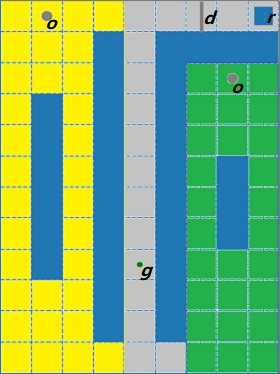
\includegraphics[width=1.2in]{simulate1/envir.png}}
\hspace{0.3in}
\subfigure[initial positions]{
\label{initial}
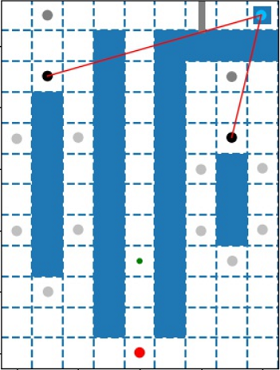
\includegraphics[width=1.2in]{simulate1/initial.png}}
\caption{(a) shows the simulation environment, where the relevant regions of different groups are in different colors and some pivotal regions are labeled. (b) shows the initial positions of agents.}
\label{first}
\end{figure}
\subsection{Task Specification}
Three different tasks are assigned to three groups of agents. The task of agents working on conveyor belts is specified as ($\square\Diamond t1 \wedge \square\Diamond t2 \wedge \square\Diamond t3 \wedge \square\Diamond t4 \wedge \square\Diamond t5 \wedge \square\Diamond t6 \wedge \square(\neg b)$) and ($\square\Diamond m1 \wedge \square\Diamond m2 \wedge \square\Diamond m3 \wedge \square\Diamond m4 \wedge \square\Diamond m5 \wedge \square\Diamond m6 \wedge \square(\neg b)$) which means that they need to often eventually bie de lun wen zen me biao shu????? visit all the checkpoints and never move across the conveyor belts. The task of agents which need to collect goods and place them in cargo collection point is specified as ???zai kan zhe ge ren wu ($\square\Diamond g \wedge \square(g\Longrightarrow \Diamond r) \wedge \square(\neg b) \wedge \square(\neg d \cup (o \wedge o'))$), which means the goods collection agents need to often eventually kan bie de lun wen zen me biao shu???????? visit $g$ and when they collect goods in $g$, they need go to $r$ to place them. The goods collection agents can never move across the belts and only when the switches are both open can they move across the door $d$. We can see $\square(\neg r \cup (o \wedge o'))$ is the compact coupled task $\varphi_c$ because it indicates that only when two switches are both open can the goods collection agents move across the door.
\subsection{Simulation Result}
The motion path of each agent is shown in Fig.\ref{path}, where different colors indicates different states of agents. The agents which are responding to deliver goods are denoted by $g_1$, they will change from red to blue when they send request message. Meanwhile, two agents are elected from $g_2$ and $g_3$ to reply the request message and change from blue to black. We record the position of agents in each time step and synthesize this motion path of agents.\par
We select two scenes to analyze the online coordination scheme. In Fig.\ref{before}, two agents, denoted by $p_0$ and $p_1$, in $g1$ are passing through the door $d$ to place the goods in goods collection point $r$. Meanwhile, two agents, denoted by $p_2$ and $p_3$, in $g_2$ and $g_3$ are elected to collaborate. $p_0$ and $p_1$ are turned to blue, and $p_2$, $p_3$ are turned to black. There are red solid lines connect $p_0$ and $p_2$, $p_3$, $p_1$ and $p_2$, $p_3$, which indicates they are transmitting message.\par
In Fig.\ref{across}, $p_0$ and $p_1$ have placed the goods in $r$ and they are going back to $g$ to collect goods. $p_0$ has passed through $d$ so it stop the sending of request message, but $p_1$ is still passing through $d$ so it continues to send the request message and $p_2$, $p_3$ continue to reply to it, so there are red solid lines connecting $p_0$ and $p_2$, $p_3$.\par
\begin{figure}
\centering
\subfigure[]{
\label{path}
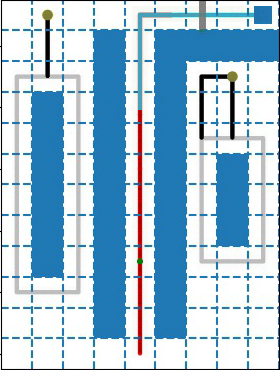
\includegraphics[width=1in]{simulate1/path.png}}
\hspace{0.02cm}
\subfigure[]{
\label{before}
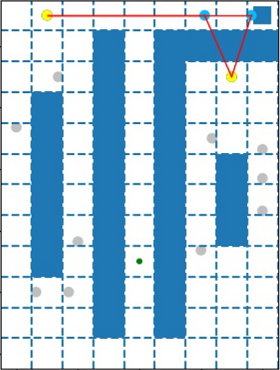
\includegraphics[width=1in]{simulate1/before.png}}
\hspace{0.02cm}
\subfigure[]{
\label{across}
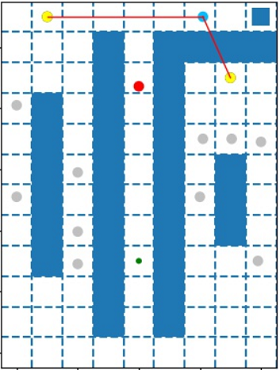
\includegraphics[width=1in]{simulate1/across.png}}
\caption{(a) shows the motion path of agents, (b) shows the message transmission when two agents are passing through the door and moving to the goods collection point and (c) shows the message transmission when two agents are going back to collect goods after they placed the goods.}
\label{second}
\end{figure}
In order to represent the collaboration of agents more intuitively, we draw the Gantt chart as Fig.\ref{Gantt}. In Fig.\ref{Gantt}, each agent has a  

\begin{figure}[h]	
\centering  	
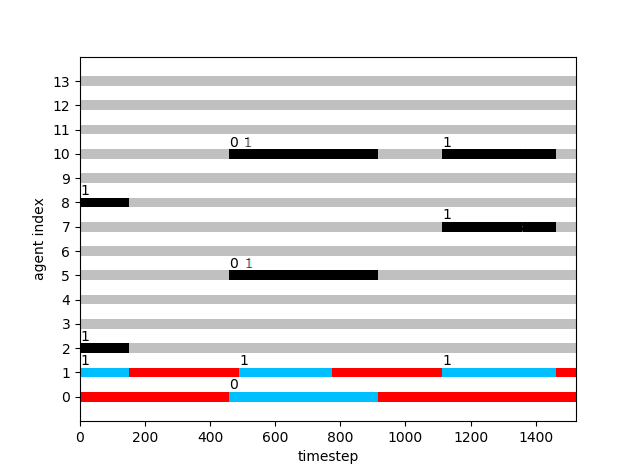
\includegraphics[width=1\linewidth]{simulate1/gante_no_grid.png}
\caption{Gantt}
\label{Gantt}
\end{figure}

\subsection{Prevention Of Long-time Demission}
\subsection{Agents Scheduling When Failure Occurs}

\section{Conclusion}
% if have a single appendix:
%\appendix[Proof of the Zonklar Equations]
% or
%\appendix  % for no appendix heading
% do not use \section anymore after \appendix, only \section*
% is possibly needed

% use appendices with more than one appendix
% then use \section to start each appendix
% you must declare a \section before using any
% \subsection or using \label (\appendices by itself
% starts a section numbered zero.)
%


%\appendices
%\section{Proof of the First Zonklar Equation}
%Appendix one text goes here.

%% you can choose not to have a title for an appendix
%% if you want by leaving the argument blank
%\section{}
%Appendix two text goes here.


% use section* for acknowledgment
\section*{Acknowledgment}


The authors would like to thank...


% Can use something like this to put references on a page
% by themselves when using endfloat and the captionsoff option.
\ifCLASSOPTIONcaptionsoff
  \newpage
\fi



% trigger a \newpage just before the given reference
% number - used to balance the columns on the last page
% adjust value as needed - may need to be readjusted if
% the document is modified later
%\IEEEtriggeratref{8}
% The "triggered" command can be changed if desired:
%\IEEEtriggercmd{\enlargethispage{-5in}}

% references section

% can use a bibliography generated by BibTeX as a .bbl file
% BibTeX documentation can be easily obtained at:
% http://mirror.ctan.org/biblio/bibtex/contrib/doc/
% The IEEEtran BibTeX style support page is at:
% http://www.michaelshell.org/tex/ieeetran/bibtex/
%\bibliographystyle{IEEEtran}
% argument is your BibTeX string definitions and bibliography database(s)
%\bibliography{IEEEabrv,../bib/paper}
%
% <OR> manually copy in the resultant .bbl file
% set second argument of \begin to the number of references
% (used to reserve space for the reference number labels box)
\begin{thebibliography}{1}

\bibitem{IEEEhowto:kopka}
H.~Kopka and P.~W. Daly, \emph{A Guide to \LaTeX}, 3rd~ed.\hskip 1em plus
  0.5em minus 0.4em\relax Harlow, England: Addison-Wesley, 1999.

\end{thebibliography}

% biography section
%
% If you have an EPS/PDF photo (graphicx package needed) extra braces are
% needed around the contents of the optional argument to biography to prevent
% the LaTeX parser from getting confused when it sees the complicated
% \includegraphics command within an optional argument. (You could create
% your own custom macro containing the \includegraphics command to make things
% simpler here.)
%\begin{IEEEbiography}[{\includegraphics[width=1in,height=1.25in,clip,keepaspectratio]{mshell}}]{Michael Shell}
% or if you just want to reserve a space for a photo:

\begin{IEEEbiography}{Michael Shell}
Biography text here.
\end{IEEEbiography}

% if you will not have a photo at all:
\begin{IEEEbiographynophoto}{John Doe}
Biography text here.
\end{IEEEbiographynophoto}

% insert where needed to balance the two columns on the last page with
% biographies
%\newpage

\begin{IEEEbiographynophoto}{Jane Doe}
Biography text here.
\end{IEEEbiographynophoto}

% You can push biographies down or up by placing
% a \vfill before or after them. The appropriate
% use of \vfill depends on what kind of text is
% on the last page and whether or not the columns
% are being equalized.

%\vfill

% Can be used to pull up biographies so that the bottom of the last one
% is flush with the other column.
%\enlargethispage{-5in}



% that's all folks
\end{document}


